% Author: Justin Yang (typeset by Jaimyn Drake)
% Email: TODO
% Spring 2025

\qns{The DTFS Fourier Basis}

\meta{\begin{itemize}
        \item First make sure that students are comfortable with the concepts of span and basis, as those will be relevant in this motivation of DTFS.
        \item With this understanding, this question aims to help students understand DTFS as a change of basis, but in the complex domain for signals.
    \end{itemize}
}

% \textbf{Learning Goal:} The goal of this problem is to get practice with inner products, norms and determining orthonormality with complex vectors. 

Recall that the entries of the DTFS Fourier Basis vectors are defined as follows:

\begin{ln-define}{DTFS Fourier Basis entry}{}
    The $n$th entry of the $k$th Fourier basis vector for a signal with period $p$ is:
    
    \[ (\mathbf{w}_k)_n = e^{i\frac{2\pi}{p}nk}= \left(e^{i\frac{2\pi}{p}}\right)^{nk} \]

\end{ln-define}


\begin{enumerate}
    \item Using the formula above, calculate the Fourier Basis vectors for $\mathbb{C}^2$.

    \ans{
        Working in $\mathbb{C}^2$ implies that our signals have a period of $p = 2$.

        Thus, we can construct our basis vectors as follows:
        $$\mathbf{w}_0 = \begin{bmatrix}
            e^{i\frac{2\pi}{2}(0)(0)} \\
            e^{i\frac{2\pi}{2}(1)(0)}
        \end{bmatrix} = \begin{bmatrix}
            e^{0} \\
            e^{0}
        \end{bmatrix} = \begin{bmatrix}
            1 \\
            1
        \end{bmatrix}$$
        $$\mathbf{w}_1 = \begin{bmatrix}
            e^{i\frac{2\pi}{2}(0)(1)} \\
            e^{i\frac{2\pi}{2}(1)(1)}
        \end{bmatrix} = \begin{bmatrix}
            e^{0} \\
            e^{i\pi}
        \end{bmatrix} = \begin{bmatrix}
            1 \\
            -1
        \end{bmatrix}$$
    }
    
    \vspace{1in}

    In order to verify your answer above, you should be able to see that the vectors you constructed are orthogonal and have a squared norm of $p =2$.

    

    \item Now that we have our Fourier Basis vectors, let's represent them as discrete-time signals of period $p = 2$. Draw a stem plot with period 2 and values corresponding to the vector elements of the Fourier basis vectors we constructed.

    \ans{
        The plot for our first basis vector $\mathbf{w}_0 = \begin{bmatrix}
            1 \\
            1
        \end{bmatrix}$ should be as follows:

        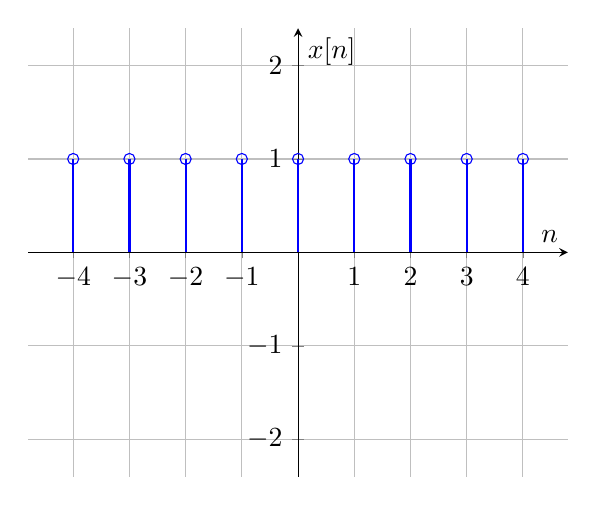
\begin{tikzpicture}
            \begin{axis}[
                axis lines=middle,
                xlabel={$n$},
                ylabel={$x[n]$},
                ymin=-2, ymax=2,
                xmin=-4, xmax=4,
                xtick={-4,-3,-2,-1,0,1,2,3,4},
                ytick={-2, -1,0,1,2},
                grid=both,
                enlargelimits=true,
            ]
                % Add vertical lines for each point in the stem plot
                \foreach \x in {-4,-3,-2,-1,0,1,2,3,4} {
                    \addplot [thick, blue] coordinates {(\x, 0) (\x, 1)};
                }
                
                % Plot markers at each stem point
                \addplot[mark=o, only marks, blue] coordinates {(-4,1) (-3,1) (-2,1) (-1,1) (0,1) (1,1) (2,1) (3,1) (4,1)};
            \end{axis}
        \end{tikzpicture}

        The plot for our second basis vector $\mathbf{w}_1 = \begin{bmatrix}
            1 \\
            -1
        \end{bmatrix}$ should be as follows:
        
        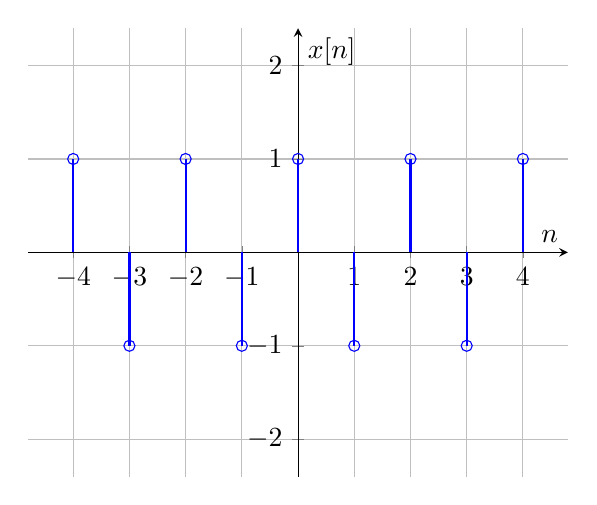
\begin{tikzpicture}
    \begin{axis}[
        axis lines=middle,
        xlabel={$n$},
        ylabel={$x[n]$},
        ymin=-2, ymax=2,
        xmin=-4, xmax=4,
        xtick={-4,-3,-2,-1,0,1,2,3,4},
        ytick={-2, -1,0,1, 2},
        grid=both,
        enlargelimits=true,
    ]
        % Add vertical lines for each point in the stem plot
        \foreach \x in {-4,-3,-2,-1,0,1,2,3,4} {
            \addplot [thick, blue] coordinates {(\x, 0) (\x, {mod(\x,2) == 0 ? 1 : -1})};
        }
        
        % Plot markers at each stem point
        \addplot[mark=o, only marks, blue] coordinates {(-4,1) (-3,-1) (-2,1) (-1,-1) (0,1) (1,-1) (2,1) (3,-1) (4,1)};
    \end{axis}
\end{tikzpicture}
    }

    \vspace{1.5in}

    \item Consider the discrete signal $x[n]$:
    
    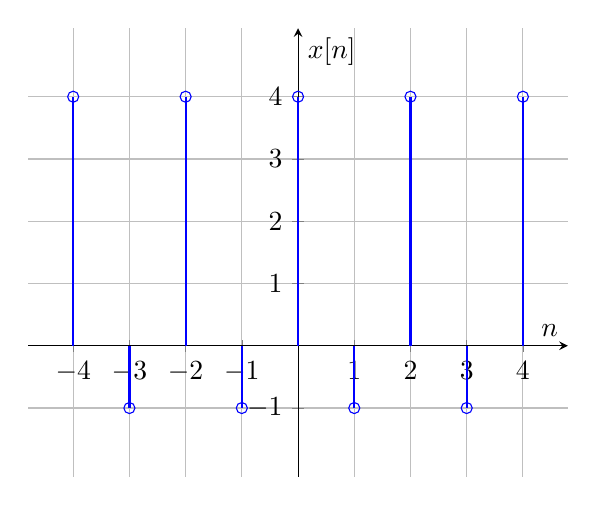
\begin{tikzpicture}
    \begin{axis}[
        axis lines=middle,
        xlabel={$n$},
        ylabel={$x[n]$},
        ymin=-1.5, ymax=4.5,
        xmin=-4, xmax=4,
        xtick={-4,-3,-2,-1,0,1,2,3,4},
        ytick={-1,0,1,2,3,4},
        grid=both,
        enlargelimits=true,
    ]
        % Add vertical lines for each point in the stem plot
        \foreach \x in {-4,-3,-2,-1,0,1,2,3,4} {
            \addplot [thick, blue] coordinates {(\x, 0) (\x, {mod(\x,2) == 0 ? 4 : -1})};
        }
        
        % Plot markers at each stem point
        \addplot[mark=o, only marks, blue] coordinates {(-4,4) (-3,-1) (-2,4) (-1,-1) (0,4) (1,-1) (2,4) (3,-1) (4,4)};
    \end{axis}
\end{tikzpicture}

    We can observe that it has period $p = 2$, so $\mathbf{x} \in \mathbb{C}^2$. In fact, we can actually represent $\mathbf{x}$ as the vector $\begin{bmatrix}
        4 \\ -1
    \end{bmatrix} \in \mathbb{C}^2$.

    Because our vector is in $\mathbb{C}^2$, we can represent it as a linear combination of our $\mathbb{C}^2$ DTFS Fourier basis vectors $\mathbf{w}_0$ and $\mathbf{w}_1$ that we derived. Find the scalar coefficients $X_0$ and $X_1$ such that:
    $$\mathbf{x} = X_0\mathbf{w}_0 + X_1\mathbf{w}_1$$

    \ans{
        We can set up our system of equations as follows:
        $$\begin{bmatrix}
            4 \\ -1 
        \end{bmatrix} = X_0\begin{bmatrix}
            1 \\ 1
        \end{bmatrix} + X_1\begin{bmatrix}
            1 \\ -1
        \end{bmatrix}$$

        This gives us:
        $$\begin{cases}
            X_0(1) + X_1(1) = 4 \\
            X_0(1) + X_1(-1) = -1
        \end{cases}$$

        From here, we can use Gaussian elimination or regular systems of equations to find that
        $$X_0 = \frac{3}{2}, \quad X_1 = \frac{5}{2}$$
    }

    \vspace{2in}

    We just did a DTFS change of basis in $\mathbb{C}^2$!  In this case, we were able to use systems of equations to find our Fourier series coefficients $X_0$ and $X_1$, but more generally they can be solved with the DTFS Analysis Equation:
    
    \begin{ln-define}{DTFS Analysis Equation}{}
    $$X_k = \frac{1}{p}\sum_{n=0}^{p-1}x[n]e^{-i\frac{2\pi}{p}nk}$$
\end{ln-define}

    \item Now, find the coefficients $X_0$ and $X_1$ again, using the DTFS Analysis Equation:

    \ans{
        \begin{align*}
            X_0 &= \frac{1}{2}\sum_{n=0}^{2-1}x[n]e^{-i\frac{2\pi}{2}n(0)} \\
            &= \frac{1}{2}\sum_{n=0}^{1}x[n]e^{0} \\
            &= \frac{1}{2}(x[0] + x[1]) \\
            &= \frac{1}{2}(4 + (-1)) \\
            &= \frac{3}{2}
        \end{align*}

        \begin{align*}
            X_1 &= \frac{1}{2}\sum_{n=0}^{2-1}x[n]e^{-i\frac{2\pi}{2}n(1)} \\
            &= \frac{1}{2}\sum_{n=0}^{1}x[n]e^{i\pi n} \\
            &= \frac{1}{2}(x[0]e^{i\pi (0)} + x[1]e^{i\pi (1)} \\
            &= \frac{1}{2}(4(1) + (-1)e^{i\pi}) \\
            &= \frac{1}{2}(4 + (-1)(-1)) \\
            &= \frac{5}{2}
        \end{align*}

        Note: Students may need some help identifying $e^{i\pi}$. In this case, using the unit circle may be helpful.
    }

    \vspace{2 in}

    Notice that we end up with the same result as our system of equations. That's because the Analysis equation is just the result of solving a system of equations written in summation form!

    In general, once we have the Fourier coefficients $X_0, X_1, \dots, X_{p-1}$ for a signal, we can reproduce the signal $x[n]$ by expressing it as a linear combination of the Fourier basis vectors. This results in the DTFS Synthesis Equation, a helpful counterpart to our DTFS Analysis Equation:

    \begin{ln-define}{DTFS Synthesis Equation}{}
    $$x[n] = \sum_{k=0}^{p-1}X_ke^{i\frac{2\pi}{p}nk}$$
\end{ln-define}
\end{enumerate}
